\documentclass[tikz]{standalone}

\colorlet{FilledSurface}{blue!20}
\colorlet{FilledSurfaceGroupOne}{blue!20}
\colorlet{FilledSurfaceGroupTwo}{red!20}
\colorlet{FilledSurfaceGroupThree}{green!20}
\colorlet{FilledSurfaceGroupFour}{magenta!20}
\colorlet{FormulaBackground}{green!10}
\colorlet{FormulaFrame}{green}


\usetikzlibrary{calc, decorations.markings, intersections, angles}

\tikzset{
    mark rect/.style={
        decoration={markings, mark=at position 0.5 with {
            \draw[draw=black, fill=white] (-6pt,-2pt) rectangle (6pt,2pt);
        }}, postaction={decorate}
    },
    mark rhombus/.style={
        decoration={
            markings,
            mark=at position 0.5 with {
                \draw[solid, fill=white] (0,5pt) -- (2pt,0) -- (0,-5pt) -- (-2pt,0) -- cycle;
            }
        },
        postaction={decorate}
    },
    mark one circle/.style={
        decoration={markings, mark=at position 0.5 with {
                \draw[fill=white] (0,0) circle (2pt);
        }}, postaction={decorate}
    },
    mark two circles/.style={
        decoration={markings, mark=at position 0.5 with {
                \draw[fill=white] (-2pt,0) circle (2pt);
                \draw[fill=white] (2pt,0) circle (2pt);
        }}, postaction={decorate}
    }
}

\begin{document}
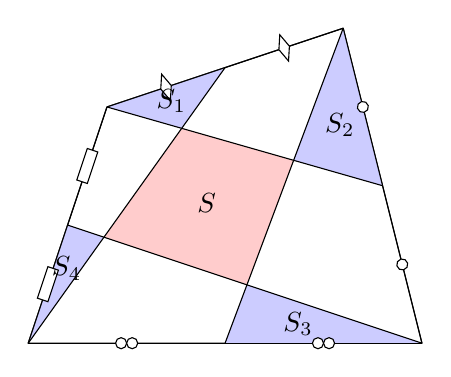
\begin{tikzpicture}

\coordinate (A) at (0, 0);
\coordinate (B) at (1, 3);
\coordinate (C) at (4, 4);
\coordinate (D) at (5, 0);

% Dibujar cuadrilátero
\draw (A) -- (B) -- (C) -- (D) -- cycle;

% Hallar puntos medios de cada lado del cuadrilátero.
\coordinate (M) at ($(A)!0.5!(B)$);
\coordinate (N) at ($(B)!0.5!(C)$);
\coordinate (P) at ($(C)!0.5!(D)$);
\coordinate (Q) at ($(D)!0.5!(A)$);

% Colorear superficies.
\path[name path = AN] (A) -- (N);
\path[name path = BP] (B) -- (P);
\path[name path = CQ] (C) -- (Q);
\path[name path = DM] (D) -- (M);

\path [name intersections={of=AN and BP, by=I1}];
\path [name intersections={of=BP and CQ, by=I2}];
\path [name intersections={of=AN and DM, by=I3}];
\path [name intersections={of=DM and CQ, by=I4}];

\fill [FilledSurfaceGroupOne] (B) -- (N) -- (I1) -- cycle;
\fill [FilledSurfaceGroupOne] (C) -- (P) -- (I2) -- cycle;
\fill [FilledSurfaceGroupOne] (Q) -- (D) -- (I4) -- cycle;
\fill [FilledSurfaceGroupOne] (A) -- (M) -- (I3) -- cycle;
\fill [FilledSurfaceGroupTwo] (I3) -- (I1) -- (I2) -- (I4) -- cycle;

% Dibujar medianas y nombrar los puntos medios de cada lado.
\path (M) -- (N) -- (P) -- (Q) -- cycle;

% Dibujar segmentos de vértices a puntos medios.
\draw (A) -- (N);
\draw (B) -- (P);
\draw (C) -- (Q);
\draw (D) -- (M);

% Añadir marcadores a los segmentos determinados por las medianas.
\draw[mark rect] (A) -- (M);
\draw[mark rect] (B) -- (M);
\draw[mark rhombus] (B) -- (N);
\draw[mark rhombus] (C) -- (N);
\draw[mark one circle] (C) -- (P);
\draw[mark one circle] (D) -- (P);
\draw[mark two circles] (D) -- (Q);
\draw[mark two circles] (A) -- (Q);

\node at (barycentric cs:B=1,N=1,I1=1) {$S_1$};
\node at (barycentric cs:C=1,P=1,I2=1) {$S_2$};
\node at (barycentric cs:Q=1,D=1,I4=1) {$S_3$};
\node at (barycentric cs:A=1,M=1,I3=1) {$S_4$};
\node at (barycentric cs:I1=1,I2=1,I3=1,I4=1) {$S$};

\end{tikzpicture}
\end{document}
